\chapter[Random Forest]{Applied Random Forest}

\begin{objetivos}
By the end of this chapter, readers should understand the Random Forest
algorithm; fit presence--background models for \textit{Dinizia excelsa};
control complexity to reduce overfitting; evaluate performance with independent
test data; compare out-of-bag (OOB) and test performance; interpret variable
importance and partial response curves; produce suitability maps; and recognize
limitations of machine-learning algorithms in SDM.
\end{objetivos}

\section{Introduction}

Random Forest is a machine-learning algorithm based on many decision trees.
Each tree is fitted to a sample of observations and a random subset of
predictors. Final predictions are obtained by averaging across trees for
regression or probability estimation, or by majority vote for classification
\parencite{breiman2001random,cutler2007random,guisan2017habitat}.

Random Forest is frequently used in SDM because it represents nonlinear
relationships, predictor interactions, and complex environmental responses.
This flexibility requires caution: a model can appear excellent on calibration
data yet generalize poorly across space or time.

\begin{conceito}[title={\faBook\quad Random Forest in SDM}]
Random Forest combines many decision trees to estimate complex relationships
between occurrence and environment. Its strength is flexibility; its risk is
overfitting when validation is not adequately controlled.
\end{conceito}

\section{Overfitting in Random Forest}

Very high metrics, such as an AUC close to 1, may indicate excellent
discrimination but can also signal overfitting, especially in the presence of
spatial autocorrelation, excessive background samples, redundant predictors, or
nonindependent validation.

Four strategies are used to reduce this risk:
\begin{itemize}
  \item a stratified training--test split;
  \item predictors retained after correlation and VIF analysis;
  \item complexity control through \texttt{mtry}, \texttt{min.node.size}, and \texttt{sample.fraction}; and
  \item comparison of OOB and test-set performance.
\end{itemize}

\begin{atencao}[title={\faExclamationTriangle\quad An extremely high AUC requires caution}]
An AUC near 1 does not necessarily identify an ecologically excellent model. It
may reflect overfitting, spatial bias, an easily distinguished background, or
nonindependent validation.
\end{atencao}

\section{Data Preparation}

The analysis uses the Chapter 5 dataset: real \textit{Dinizia excelsa}
presences, background sampled within $M$, and predictors retained in Chapter 4.

\rscriptfile{scripts/unidade08/01_estrutura_pastas.R}
\rscriptfile{scripts/unidade08/02_preparar_dados_rf.R}

\section{Controlled Random Forest Fitting}

The model is fitted with \texttt{ranger}, using its probability-forest output.
Because the contrast class is background rather than confirmed absence, this
numeric output is interpreted as a relative score, not absolute occurrence
probability.
Moderate \texttt{mtry}, a larger-than-default \texttt{min.node.size}, and a
\texttt{sample.fraction} below 1 constrain complexity.

\rscriptfile{scripts/unidade08/03_ajustar_rf_dinizia.R}

\begin{figure}[H]
  \centering
  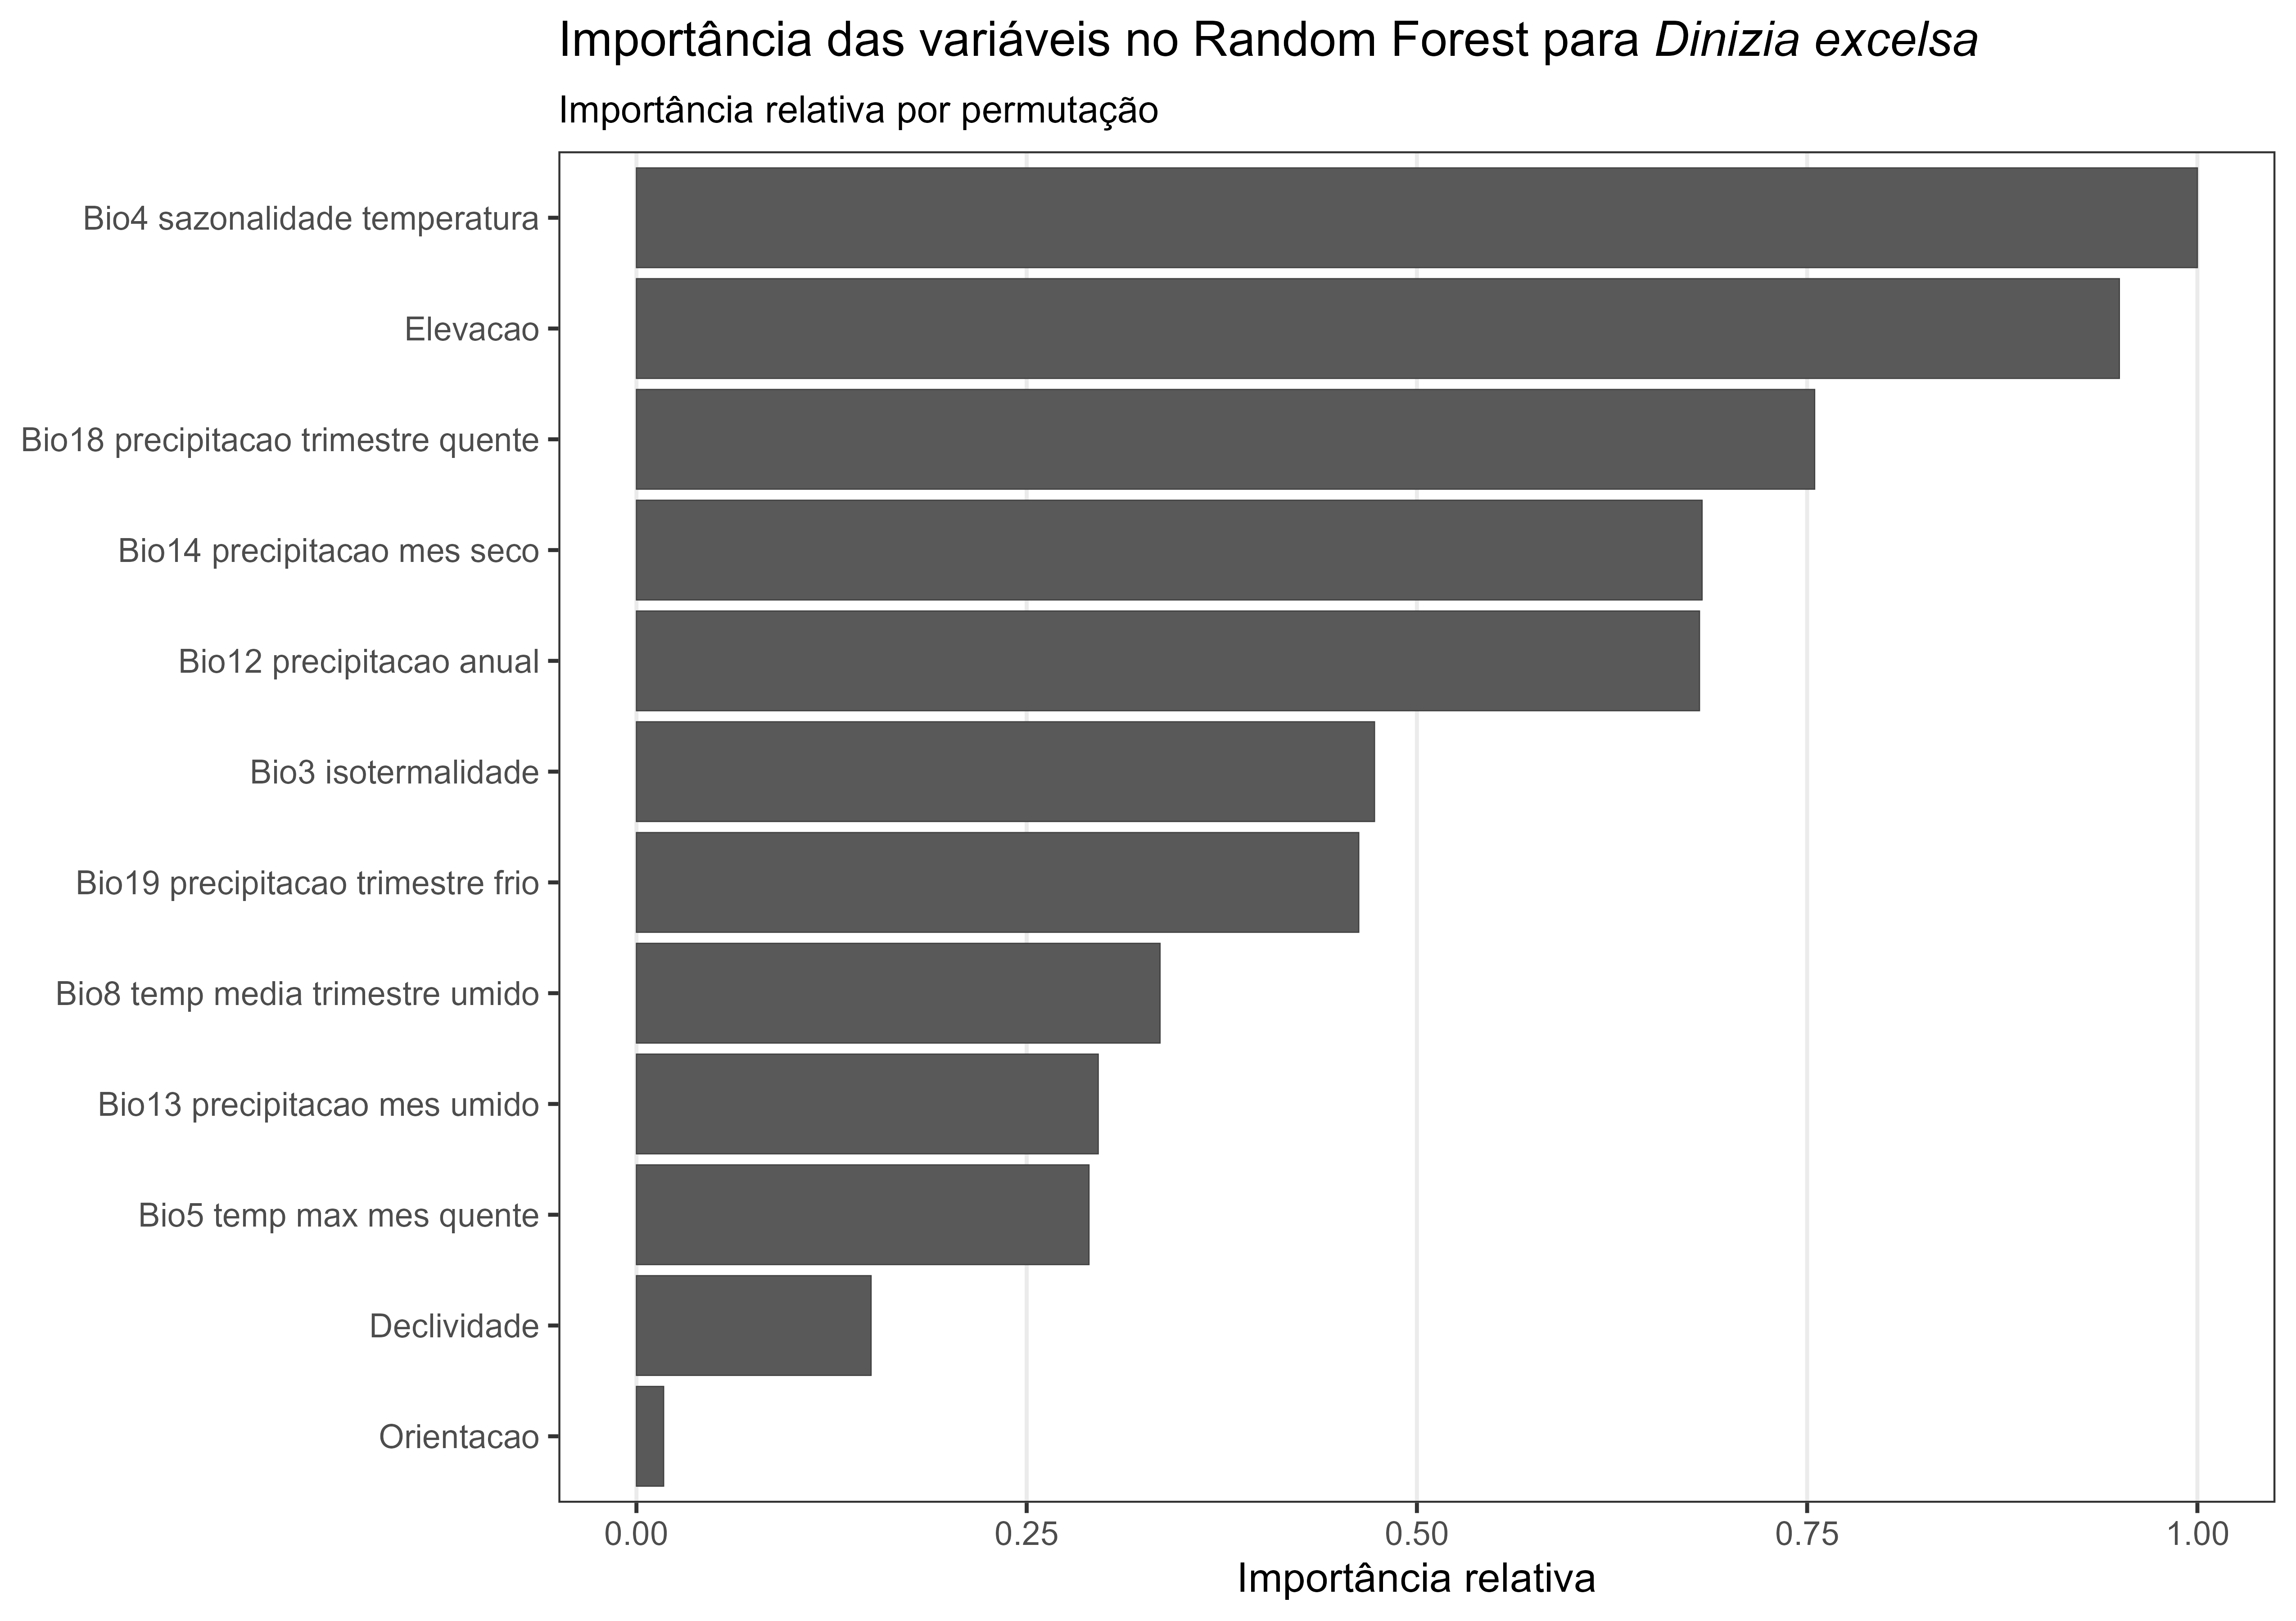
\includegraphics[width=0.86\textwidth]{figuras/unidade08/unidade08_importancia_variaveis_rf.png}
  \caption{Environmental-predictor importance in the Random Forest fitted to \textit{Dinizia excelsa}.}
  \label{fig:unidade08_importancia_rf}
\end{figure}

\section{Model Evaluation}

Performance is evaluated on the test set rather than the training data. OOB AUC
and test AUC are also compared; large differences may indicate instability or
overfitting.

\rscriptfile{scripts/unidade08/04_avaliar_rf_dinizia.R}

\begin{figure}[H]
  \centering
  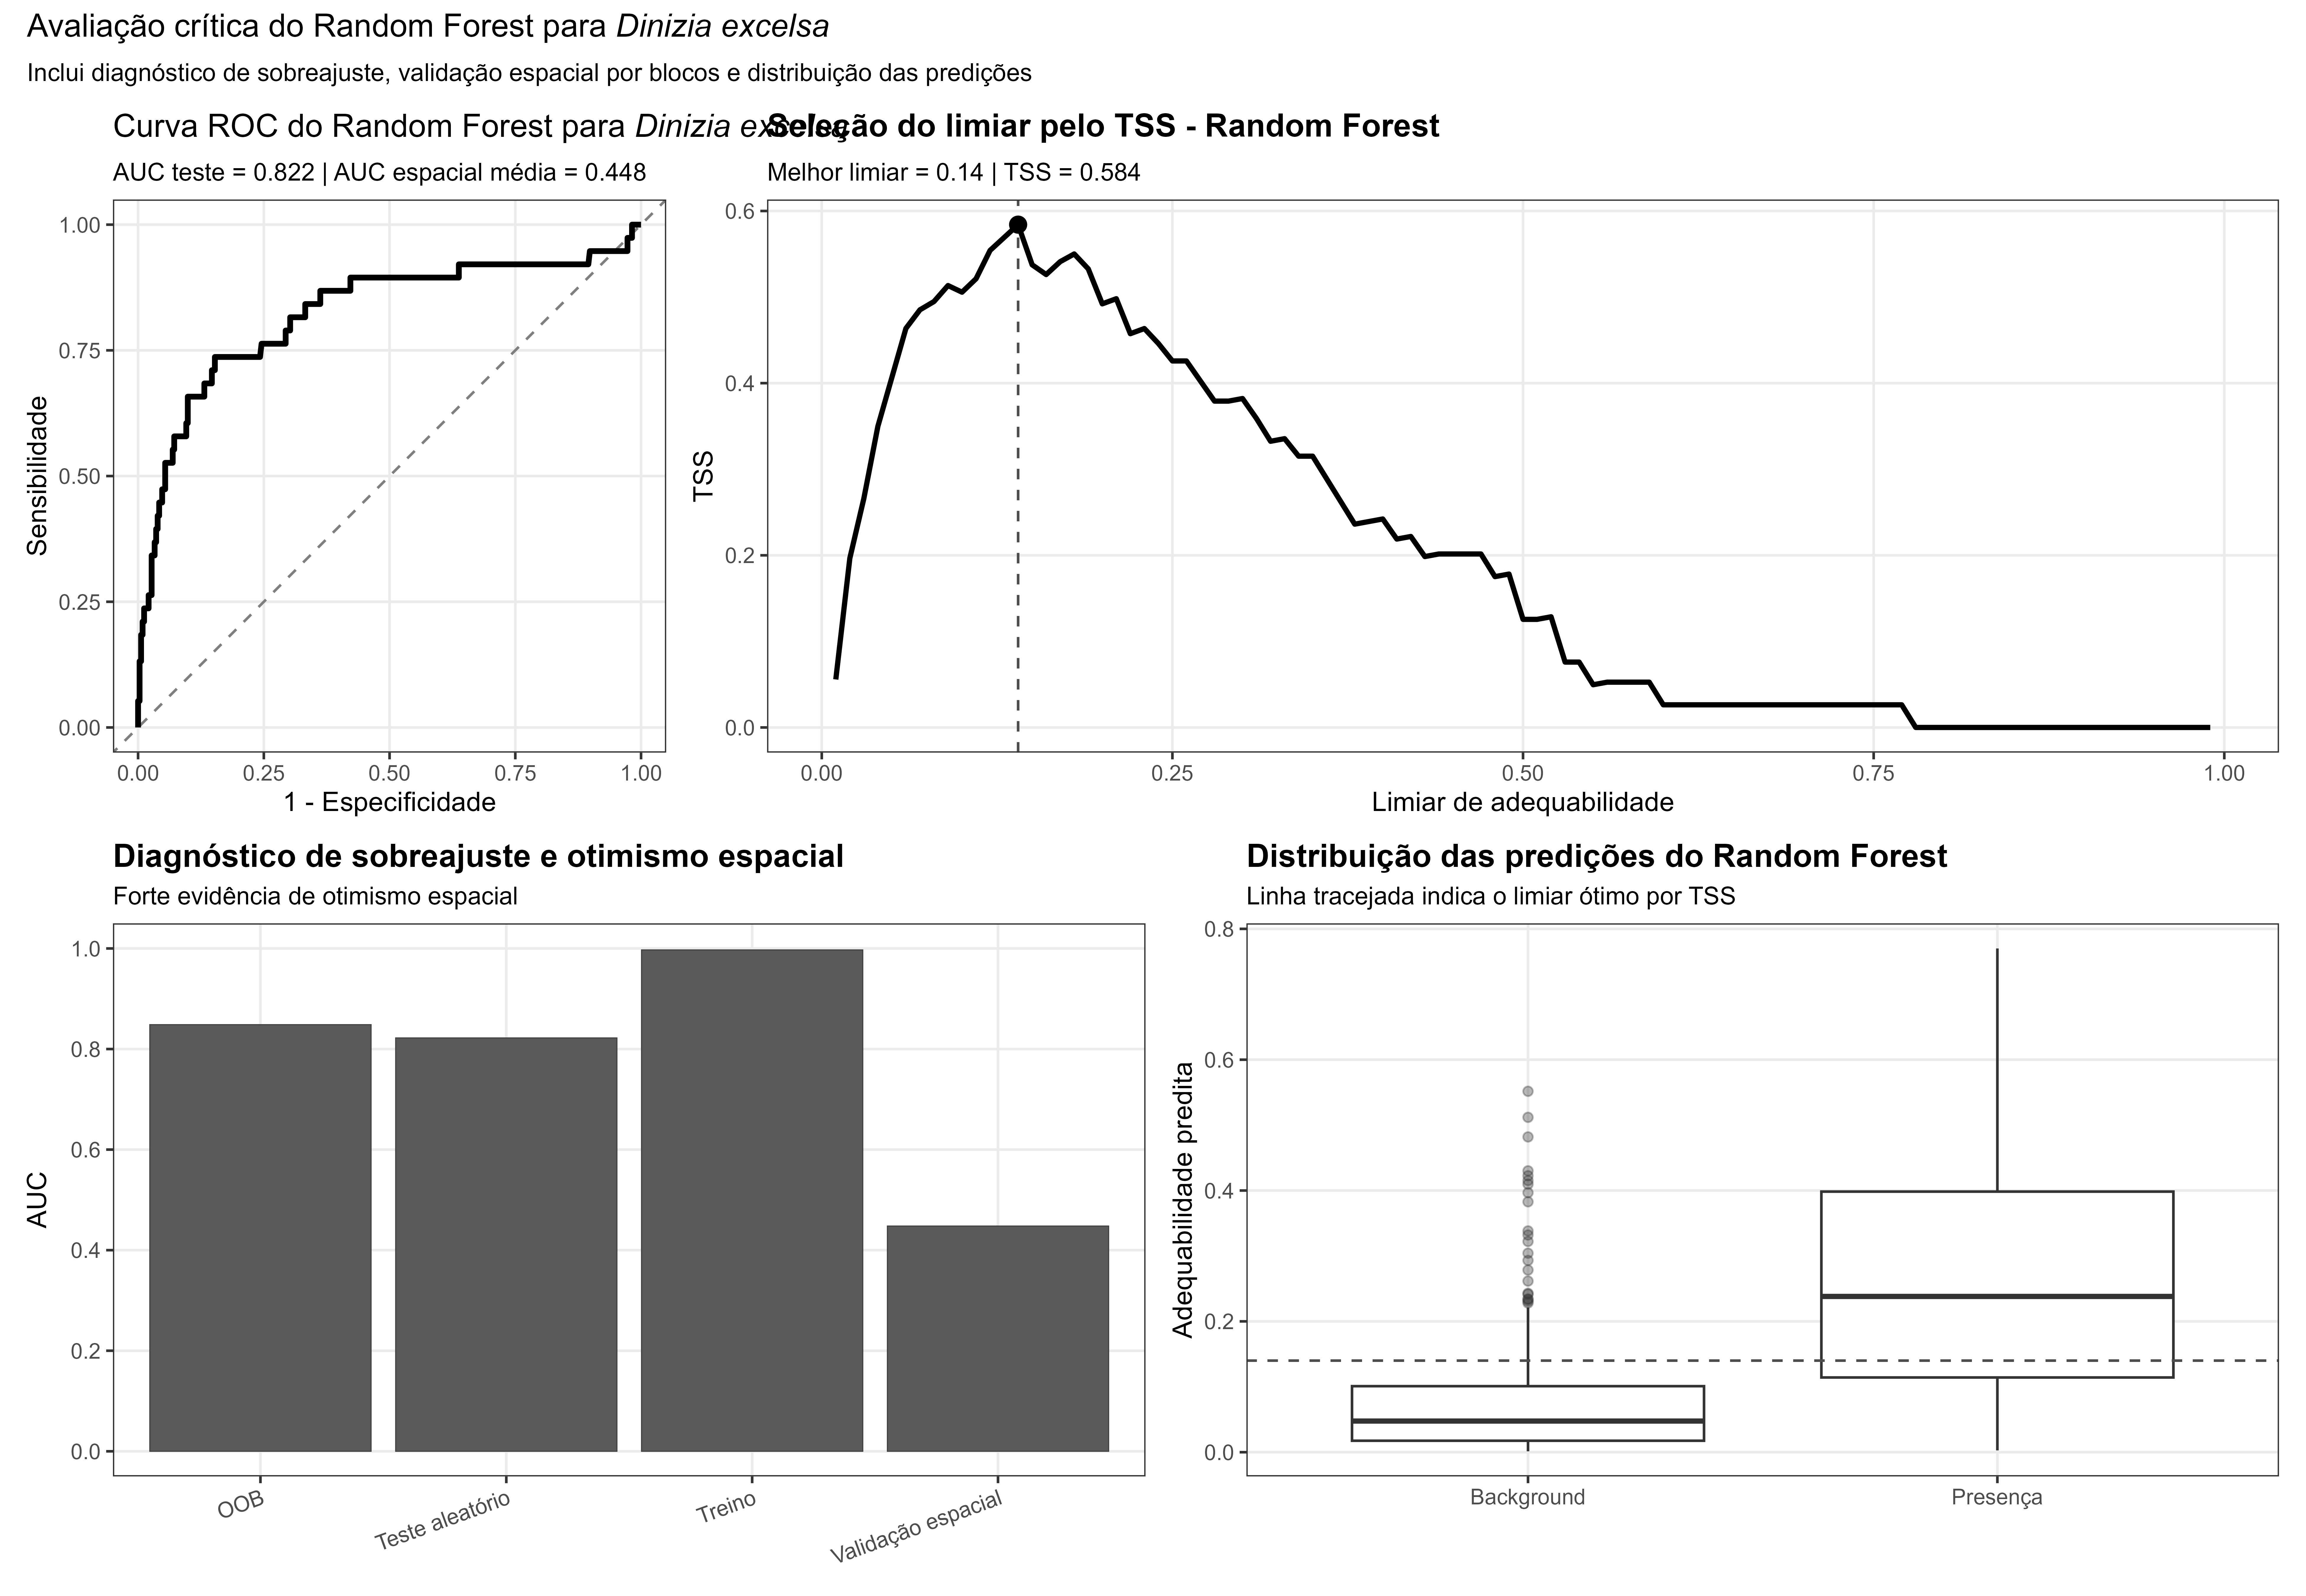
\includegraphics[width=0.78\textwidth]{figuras/unidade08/unidade08_avaliacao_rf_patchwork.png}
  \caption{ROC curve for the Random Forest evaluated on the test set.}
  \label{fig:unidade08_roc_rf}
\end{figure}

\section{Current Suitability Map}

After evaluation, the model is projected across $M$ to produce a continuous
map of current environmental suitability.

\rscriptfile{scripts/unidade08/05_predicao_espacial_rf.R}

\begin{figure}[H]
  \centering
  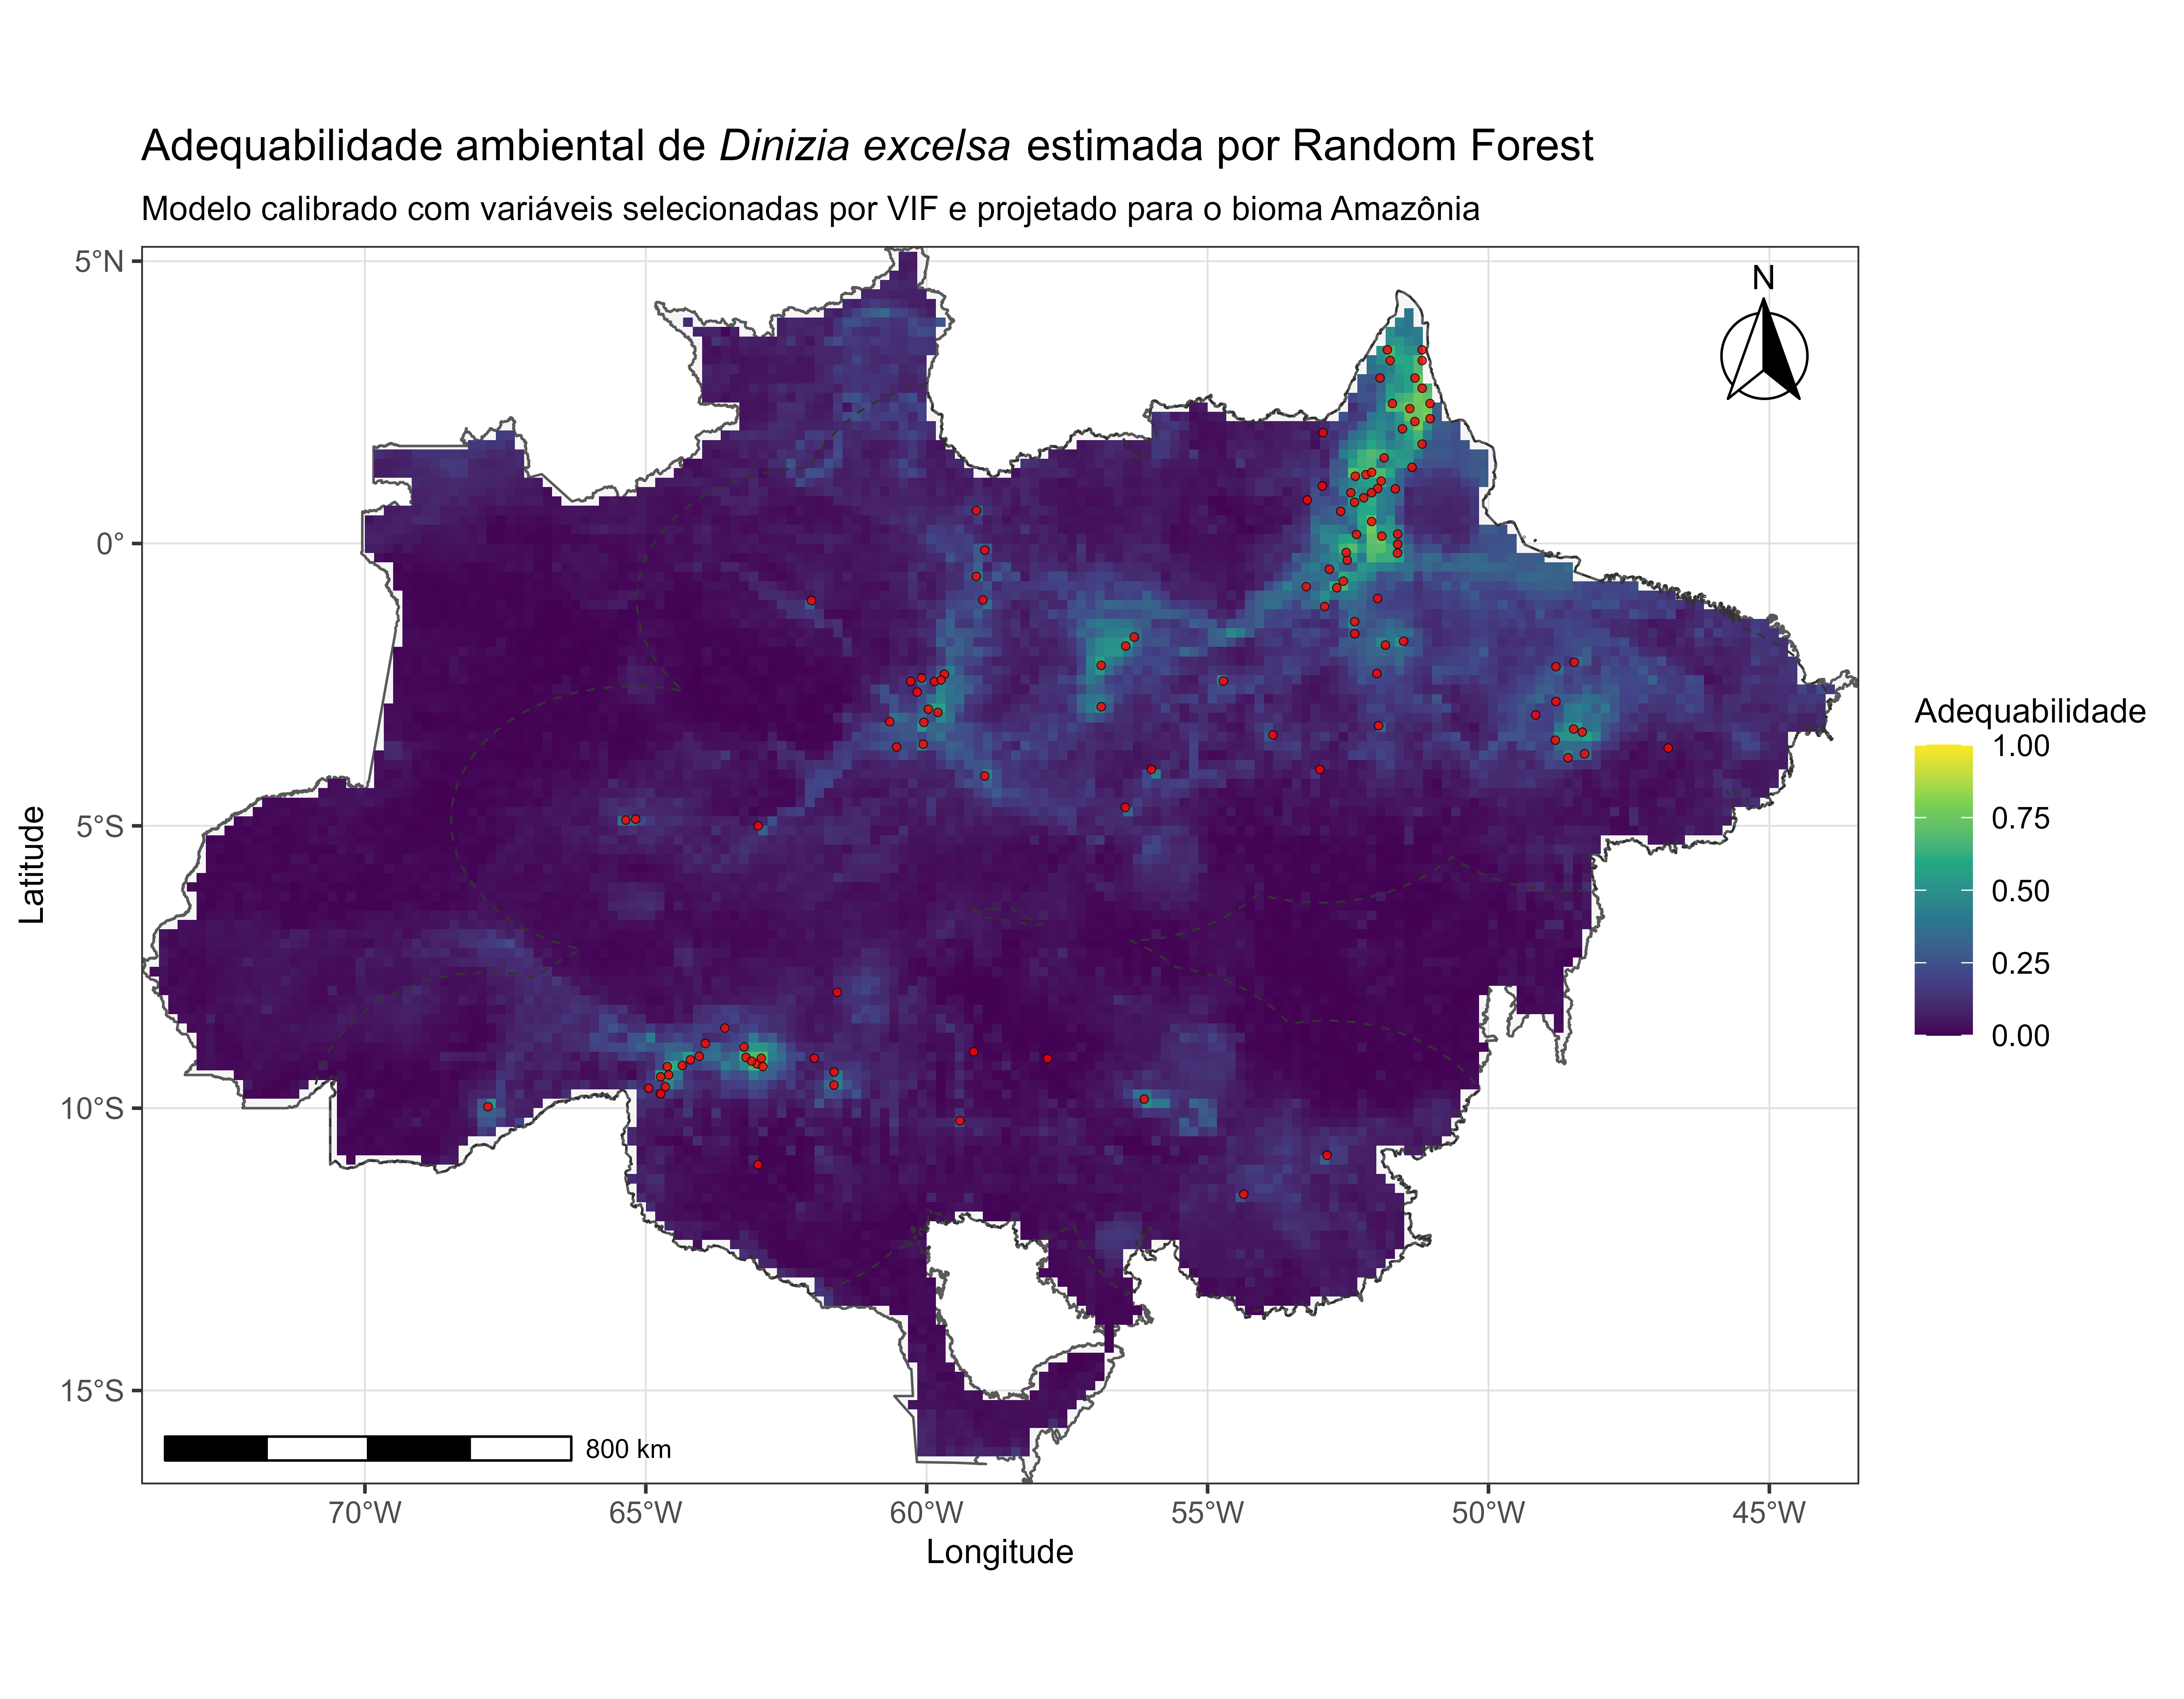
\includegraphics[width=0.88\textwidth]{figuras/unidade08/unidade08_adequabilidade_rf.png}
  \caption{Current environmental suitability for \textit{Dinizia excelsa} estimated by Random Forest within $M$.}
  \label{fig:unidade08_adequabilidade_rf}
\end{figure}

\begin{figure}[H]
  \centering
  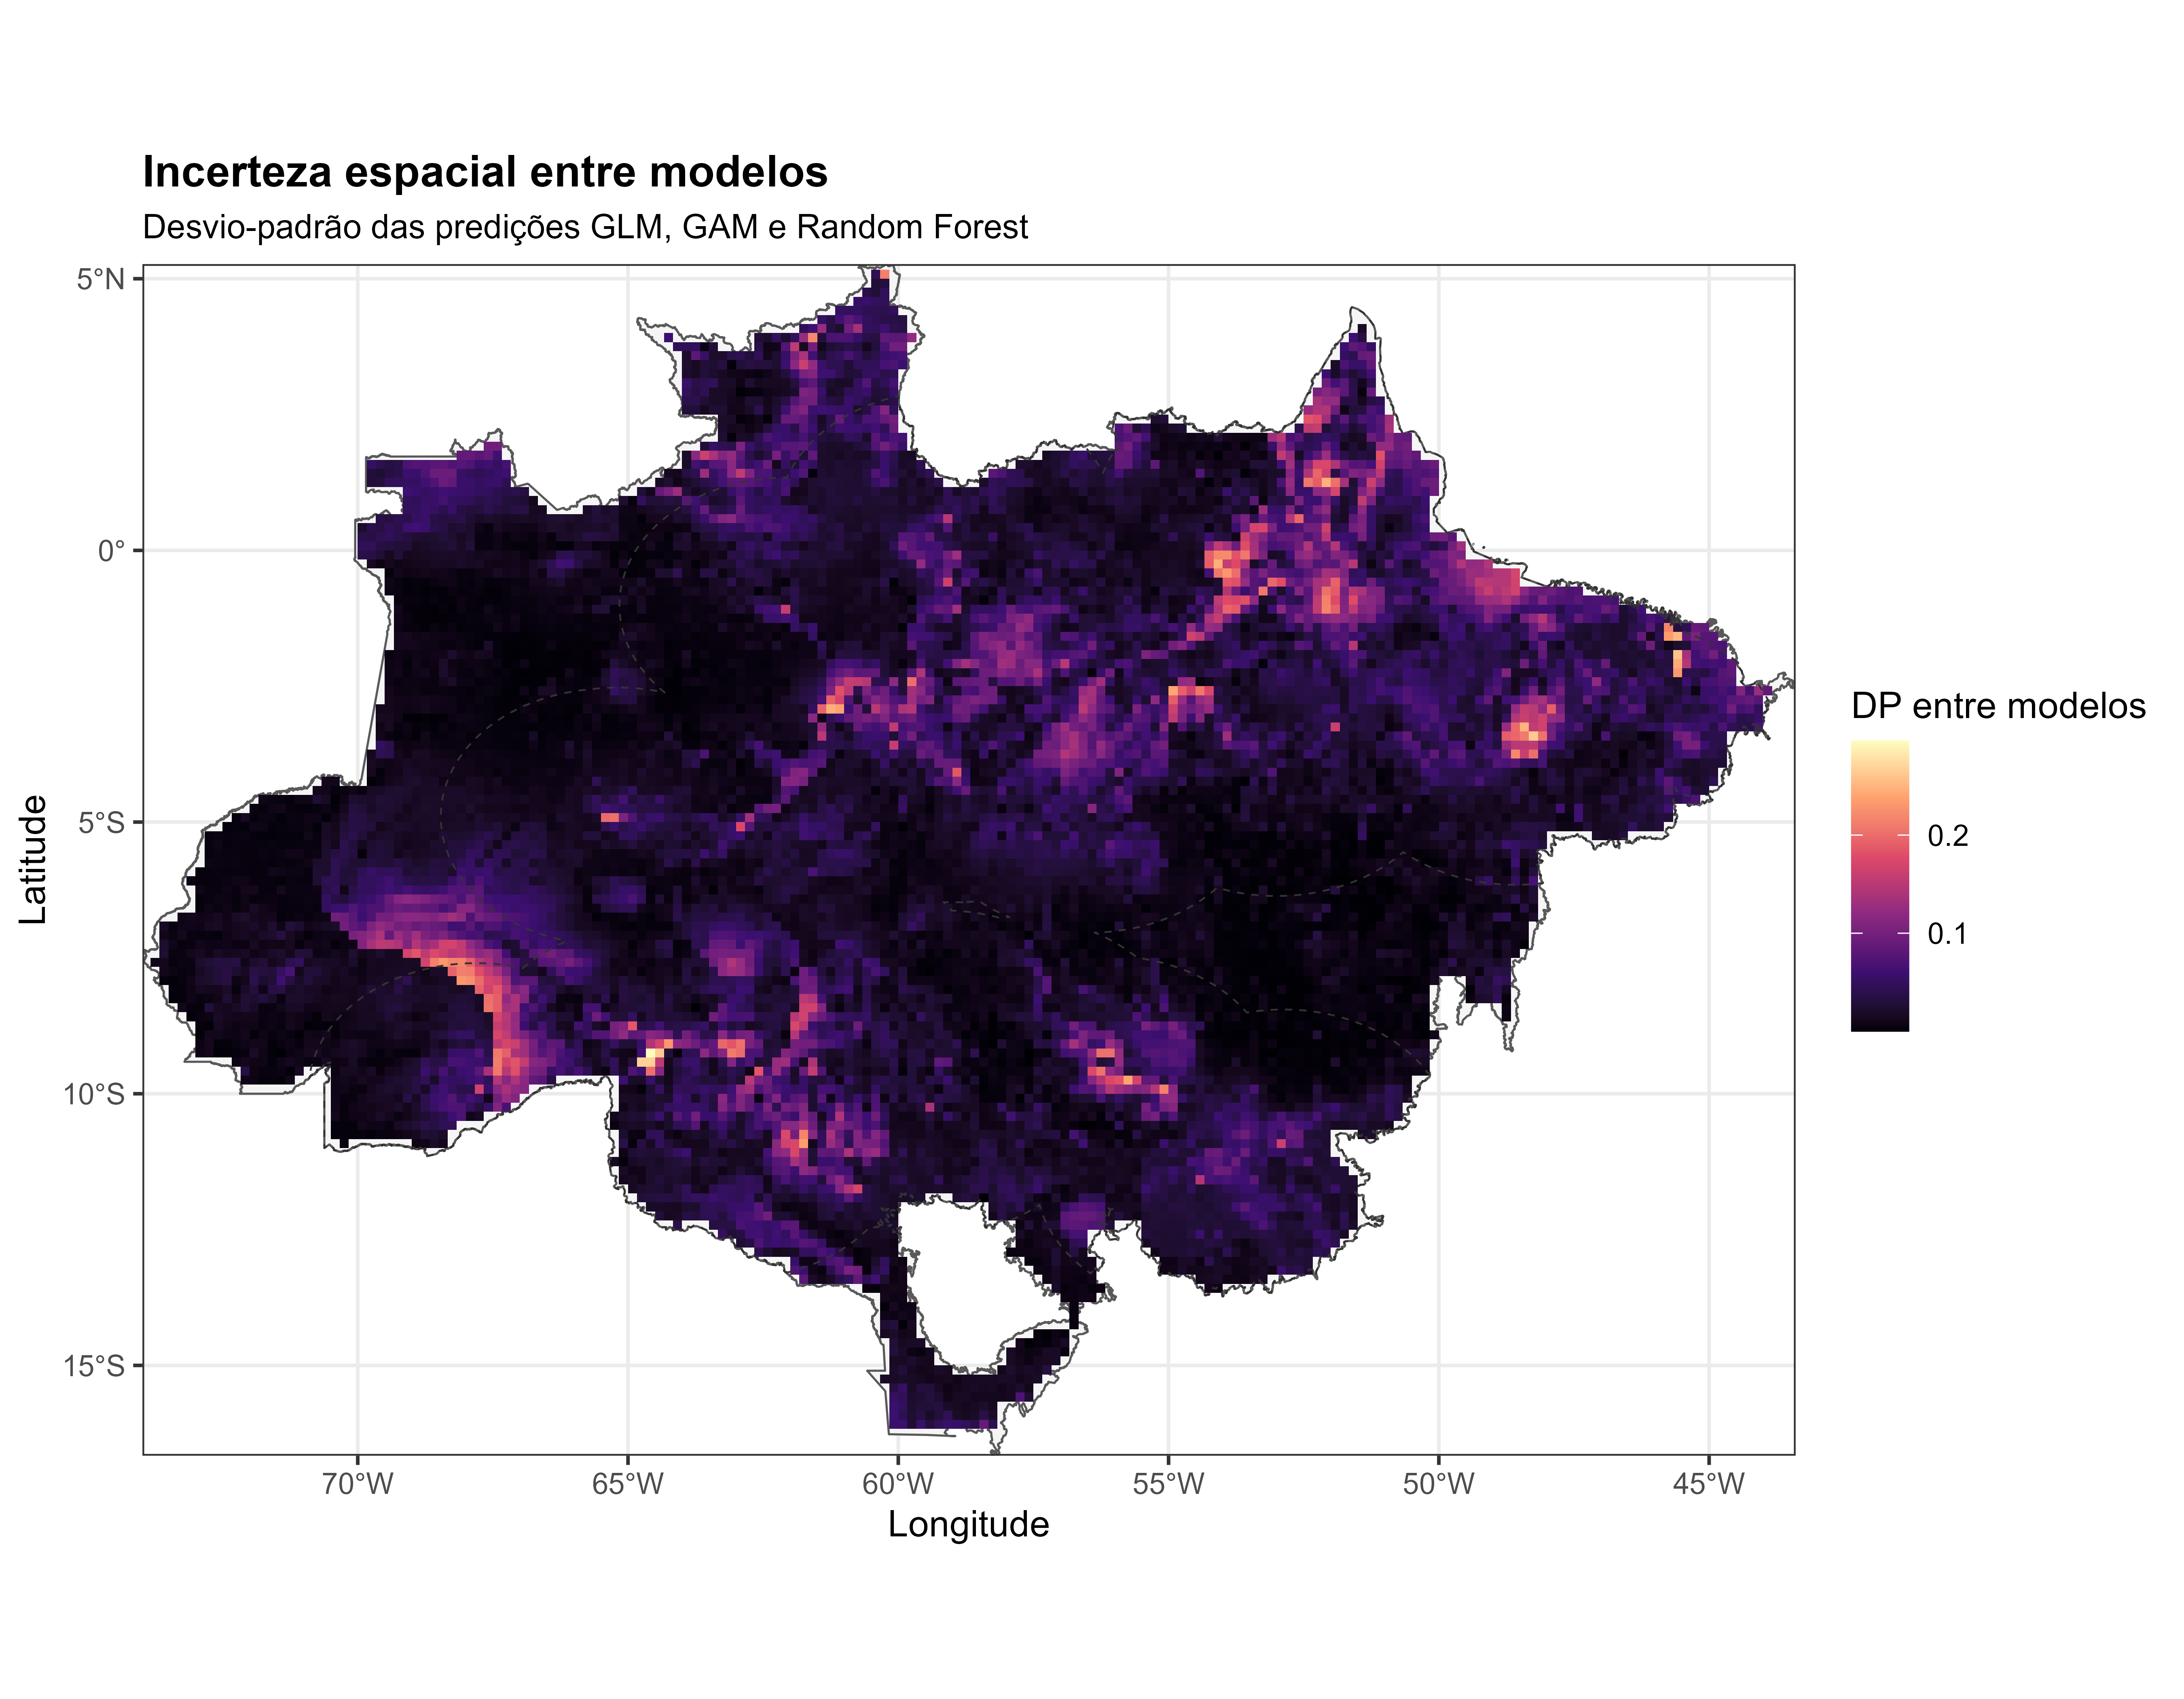
\includegraphics[width=0.78\textwidth]{figuras/unidade08/unidade08_incerteza_sd_glm_gam_rf.png}
  \caption{Spatial uncertainty measured as the standard deviation among GLM, GAM, and Random Forest predictions. High values indicate greater algorithmic disagreement; low values indicate stronger consensus.}
  \label{fig:unidade08_incerteza_modelos}
\end{figure}

\section{Partial Response Curves}

Partial dependence supports ecological interpretation. These curves are not
direct coefficients; they summarize the average prediction as one predictor
varies while the others are held constant.

\rscriptfile{scripts/unidade08/06_curvas_resposta_rf.R}

\begin{figure}[H]
  \centering
  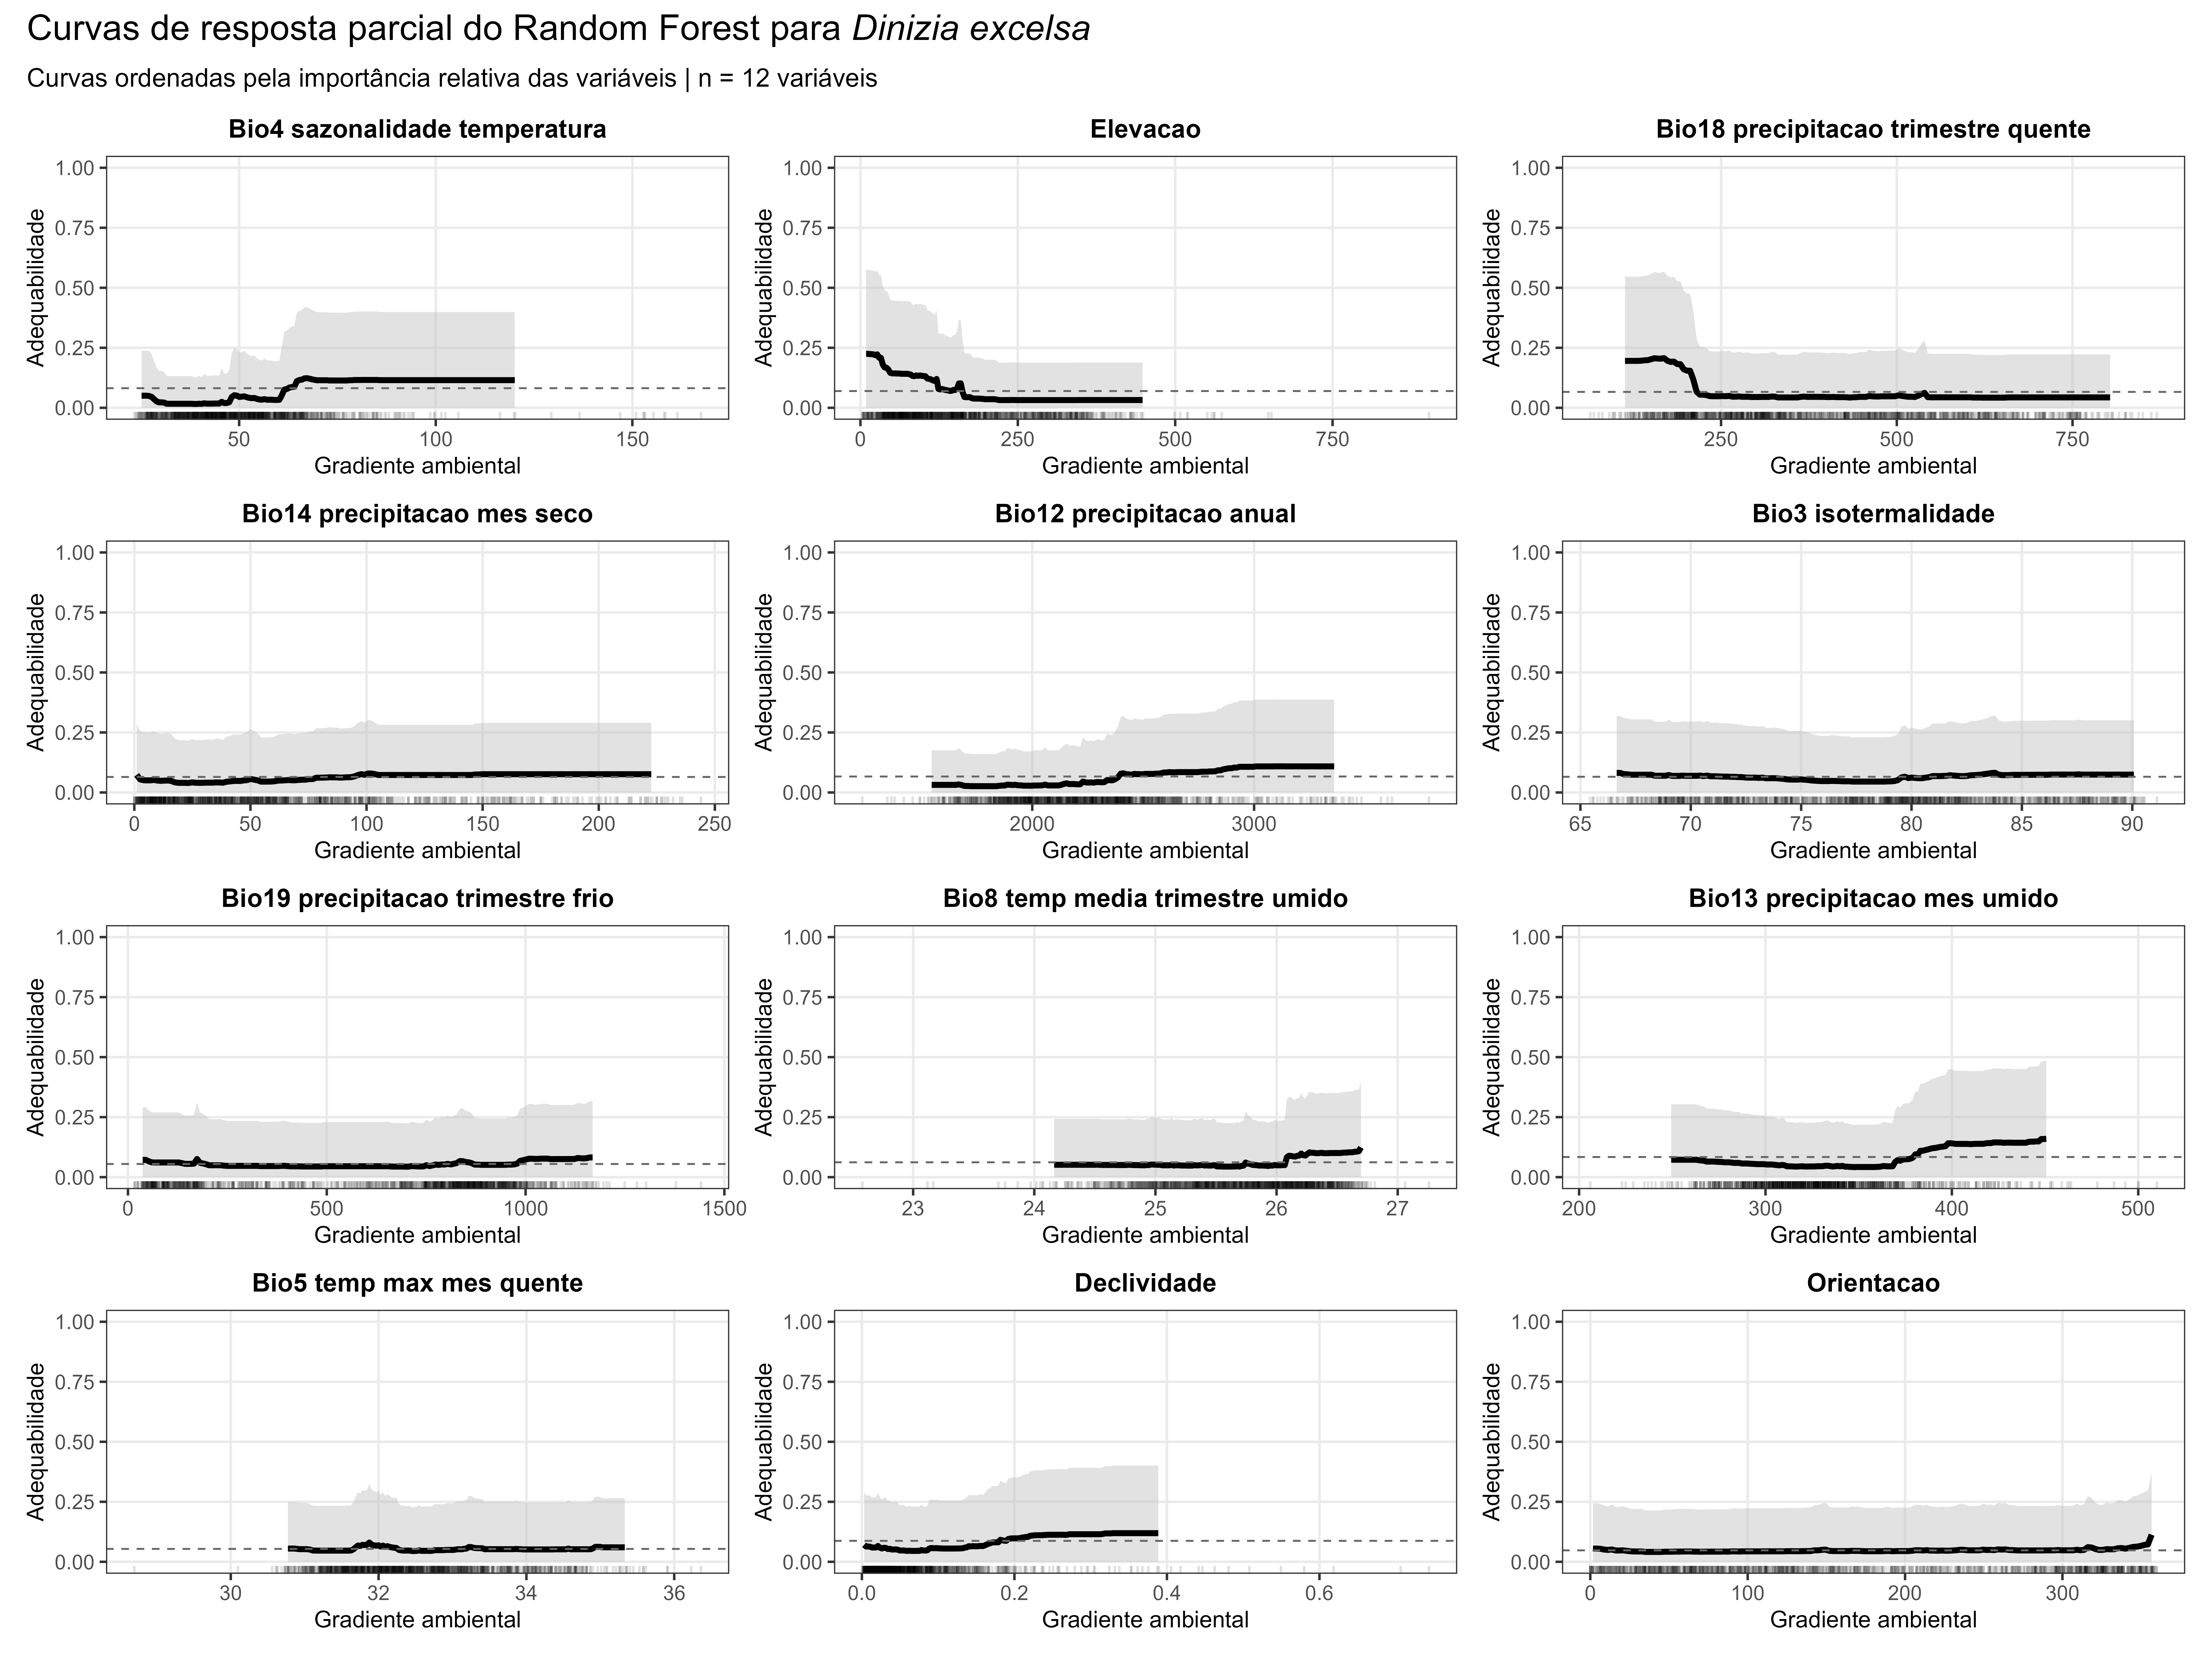
\includegraphics[width=0.96\textwidth]{figuras/unidade08/unidade08_curvas_resposta_rf.png}
  \caption{Random Forest partial response curves for the selected environmental predictors.}
  \label{fig:unidade08_curvas_resposta_rf}
\end{figure}

\section{Comparison with GLM and GAM}

The Random Forest map is compared with GLM and GAM projections, illustrating
how algorithms with different flexibility can produce distinct spatial patterns.

\rscriptfile{scripts/unidade08/07_comparar_glm_gam_rf.R}

\begin{figure}[H]
  \centering
  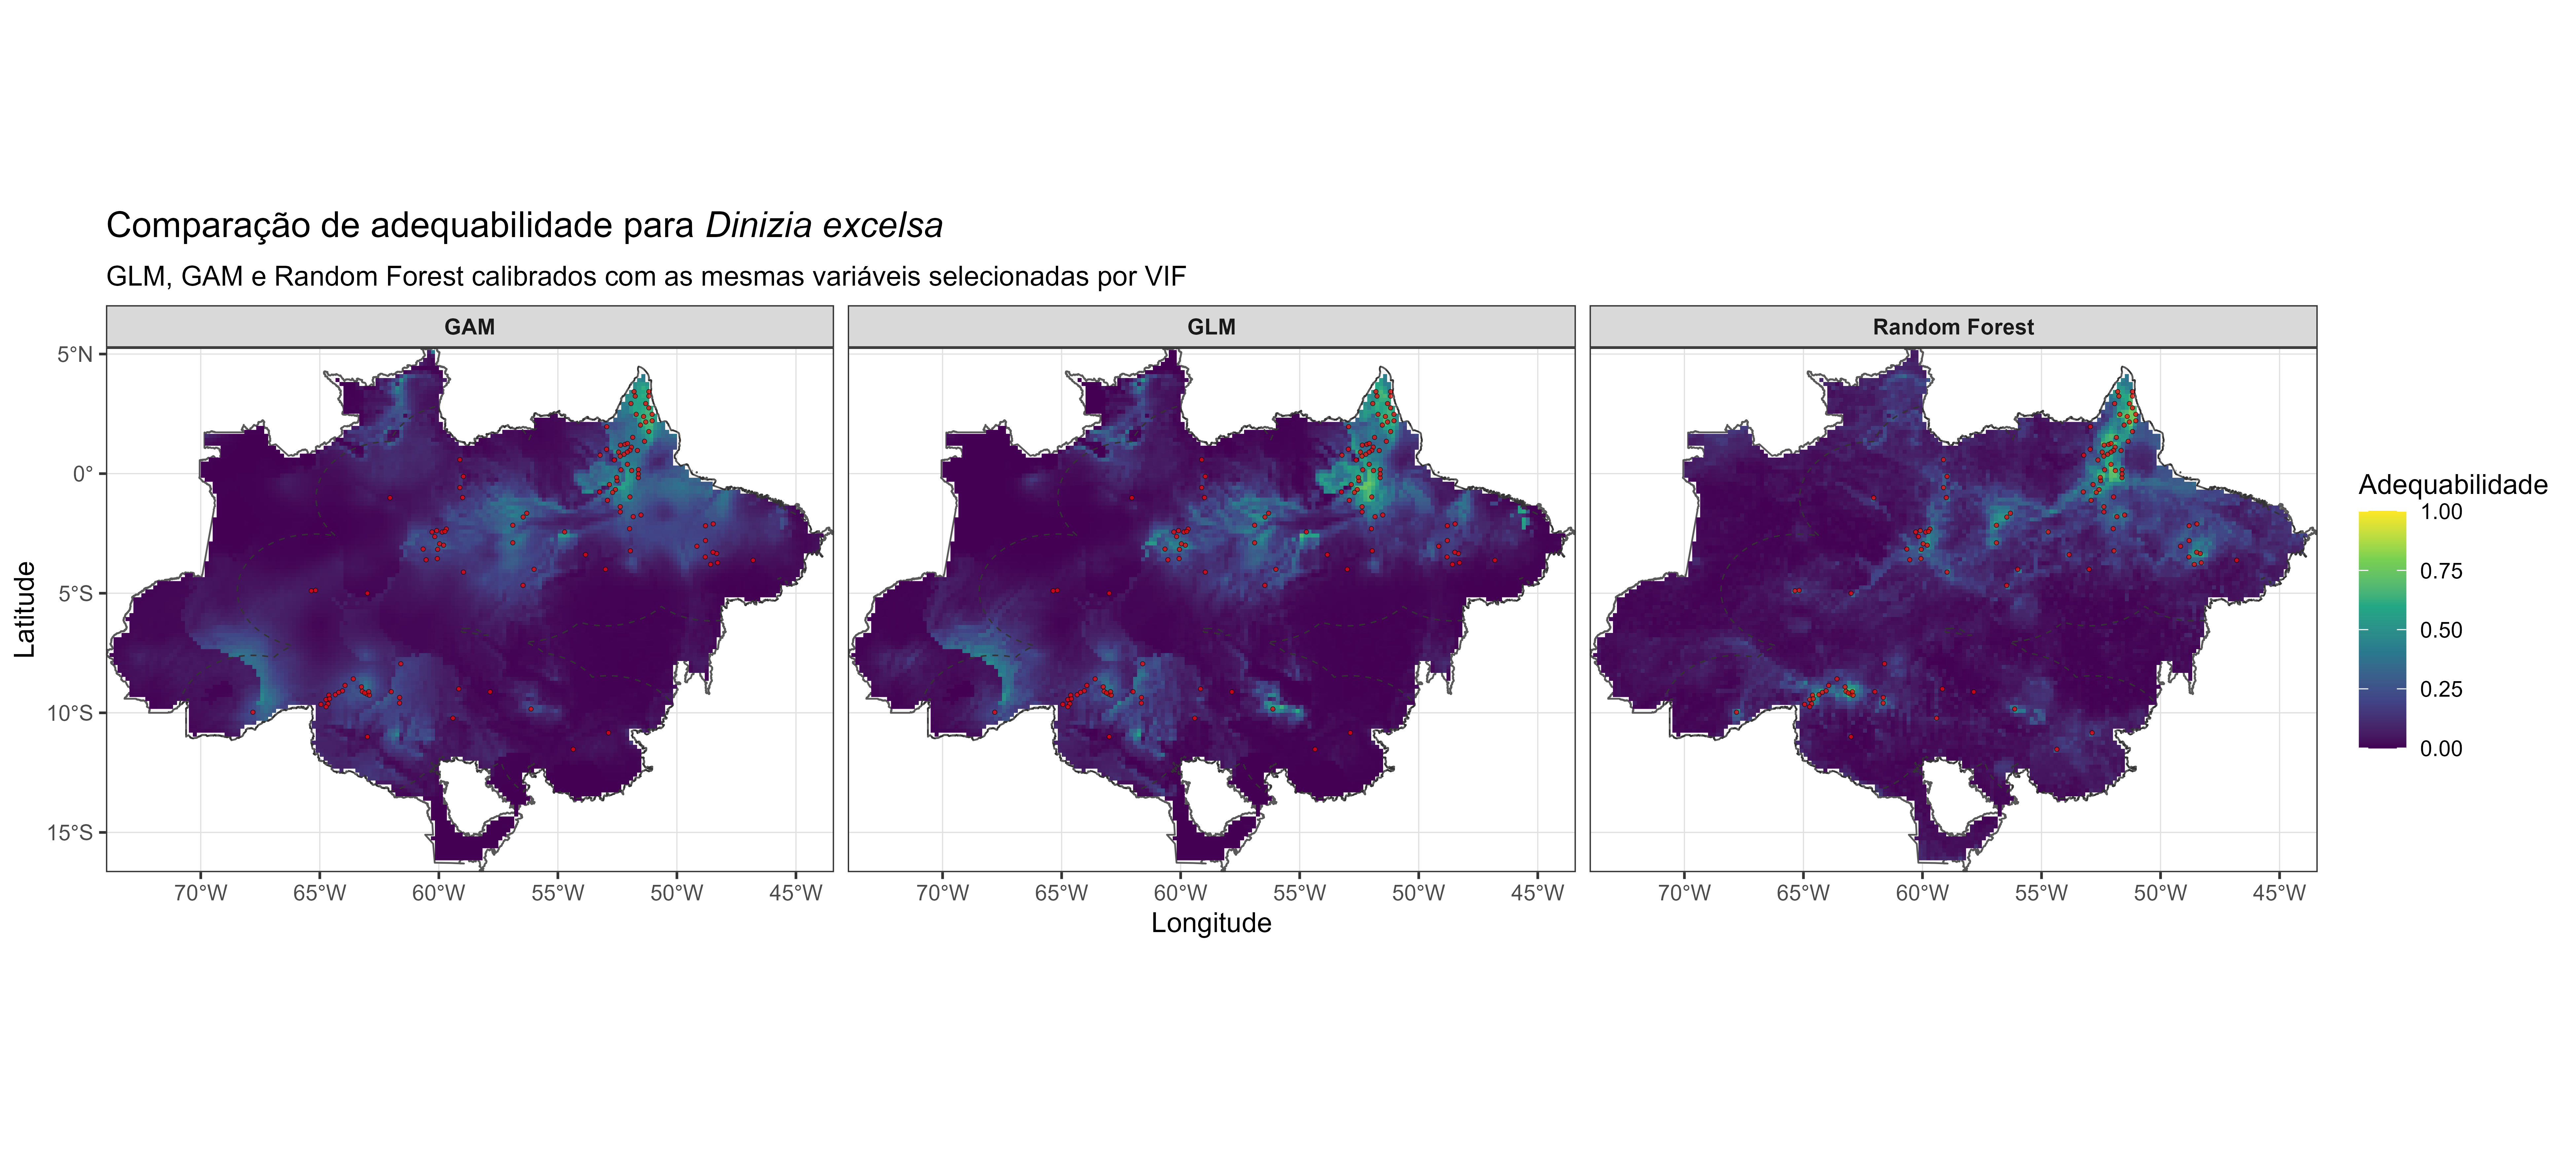
\includegraphics[width=0.96\textwidth]{figuras/unidade08/unidade08_comparacao_glm_gam_rf.png}
  \caption{Comparison of suitability maps estimated by GLM, GAM, and Random Forest.}
  \label{fig:unidade08_comparacao_modelos}
\end{figure}

\section{Complete Pipeline}
\rscriptfile{scripts/unidade08/08_pipeline_rf.R}

\section{Chapter Summary}

Random Forest is powerful when environmental relationships are nonlinear and
interactions are important. It nevertheless requires careful validation. High
metrics must be interpreted alongside overfitting diagnostics, ecological
coherence, response curves, spatial prediction patterns, and comparisons with
simpler models.

\begin{conceito}[title={\faBook\quad Key message}]
Random Forest may improve predictive performance, but it does not replace
ecological reasoning. A complex model is useful only when it generalizes,
produces plausible responses, and is evaluated independently.
\end{conceito}

\section{Review Exercises}
\begin{enumerate}
  \item Explain how Random Forest combines multiple decision trees.
  \item Why can Random Forest capture nonlinear relationships?
  \item What is overfitting in SDM?
  \item Why can an extremely high AUC be concerning?
  \item Distinguish OOB from test-set performance.
  \item What are the roles of \texttt{mtry}, \texttt{min.node.size}, and \texttt{sample.fraction}?
  \item How do partial response curves support interpretation of Random Forest?
\end{enumerate}
